\documentclass[twoside]{article}

\usepackage{amsfonts,amssymb,amsbsy,textcomp,marvosym,amsmath,caption,threeparttable,amsthm,subfigure}
\usepackage{eurosym,mathrsfs,fancyhdr,CJK,multicol,graphics,indentfirst,color,bm,upgreek,booktabs,graphicx}
\usepackage{amsmath,amsfonts,amssymb}
\usepackage{amsthm}
\usepackage{setspace}
\usepackage{algpseudocode}
\usepackage[linesnumbered,boxed,ruled,commentsnumbered]{algorithm2e}
\usepackage{graphicx}
\usepackage{xspace}
\looseness=-1
%------------Page layout and margin and Headrule-------------
\headsep=5mm \headheight=4mm \topmargin=0cm \oddsidemargin=-0.5cm
\evensidemargin=-0.5cm \marginparwidth=0pt \marginparsep= 0pt
\marginparpush=0pt \textheight=23.1cm \textwidth=17.5cm \footskip=8mm
\columnsep=7mm \setlength{\doublerulesep}{0.1pt}
\renewcommand{\thefootnote}{\fnsymbol{footnote}}
\footnotesep=3.5mm\arraycolsep=2pt
\font\tenrm=cmr10
%===========================================================
\def\footnoterule{\kern 1mm \hrule width 10cm \kern 2mm}
\def\rmd{{\rm d}} \def\rmi{{\rm i}} \def\rme{{\rm e}}
\def\sj#1{$^{[#1]}$}\def\lt{\left}\def\rt{\right}
\renewcommand{\captionfont}{\footnotesize}
\renewcommand\tablename{\bf \footnotesize Table}
\renewcommand\figurename{\footnotesize Fig.\!\!}
\captionsetup{labelsep=period}%
\allowdisplaybreaks
\sloppy
\renewcommand{\headrulewidth}{0pt}
\catcode`@=11
\def\title#1{\vspace{3mm}\begin{flushleft}\vglue-.1cm\Large\bf\boldmath\protect\baselineskip=18pt plus.2pt minus.1pt #1
\end{flushleft}\vspace{1mm} }
\def\author#1{\begin{flushleft}\normalsize #1\end{flushleft}\vspace*{-4pt} \vspace{3mm}}
\def\address#1#2{\begin{flushleft}\vglue-.35cm${}^{#1}$\small\it #2\vglue-.35cm\end{flushleft}\vspace{-2mm}\par}
\def\jz#1#2{{$^{\footnotesize\textcircled{\tiny #1}}$\footnotetext{$^{\footnotesize\textcircled{\tiny #1}}$#2}}}
\def\jzd#1#2{$^{\footnotesize\textcircled{\tiny{#1}}}$\footnotetext{$^{\footnotesize\textcircled{\tiny{#1}}}$#2}}
\catcode`@=11
\def\section{\@startsection{section}{1}{\z@}%
 %{-3.5ex \@plus -1ex \@minus -.2ex}%
 {-3ex \@plus -.3ex \@minus -.2ex}%
 {2.2ex \@plus.2ex}%
{\normalfont\normalsize\protect\baselineskip=14.5pt plus.2pt minus.2pt\bfseries}}
\def\subsection{\@startsection{subsection}{2}{\z@}%
 %{-3.25ex\@plus -1ex \@minus -.2ex}%
 {-3ex\@plus -.2ex \@minus -.2ex}%
 {2ex \@plus.2ex}%
{\normalfont\normalsize\protect\baselineskip=12.5pt plus.2pt minus.2pt\bfseries}}
\def\subsubsection{\@startsection{subsubsection}{3}{\z@}%
 %{-3.25ex\@plus -1ex \@minus -.2ex}%
 {-2.2ex\@plus -.21ex \@minus -.2ex}%
 {1.4ex \@plus.2ex}
{\normalfont\normalsize\protect\baselineskip=12pt plus.2pt minus.2pt\sl}}
\def\proofname{{\indent \it Proof.}}
%===========================================================ÒÔÉϲ»¶¯

\newtheorem{theorem}{Theorem}
\newtheorem{lemma}{Lemma}
\newtheorem{corollary}{Corollary}
\newtheorem{definition}{Definition}

\newcommand\ltl{\textsf{LTL}\xspace}
\newcommand\ltlf{\textsf{LTL}$_f$\xspace}
\renewcommand{\tt}{{\sf tt}\xspace}
\newcommand{\ff}{{\sf ff}\xspace}
\newcommand{\X}{\mathcal{X}}
\newcommand{\N}{\mathcal{N}}
\newcommand{\U}{\mathcal{U}}
\newcommand{\R}{\mathcal{R}}
\newcommand{\G}{\Box}
\newcommand{\F}{\Diamond}
\newcommand{\cf}{{\sf CF}\xspace}
\newcommand{\cl}{{\sf cl}\xspace}
\newcommand{\PA}{{\sf PA}\xspace}
\newcommand{\A}{\mathcal{A}}
\newcommand{\SAT}{{\sf SAT}\xspace}
\newcommand{\NFA}{{\sf NFA}\xspace}
\newcommand{\TNFA}{{\sf TNFA}\xspace}
\newcommand{\DFA}{{\sf DFA}\xspace}
\newcommand{\TDFA}{{\sf TDFA}\xspace}
\newcommand{\XNF}{{\sf XNF}\xspace}
\newcommand{\NNF}{{\sf NNF}\xspace}
\newcommand{\xnf}{{\sf xnf}\xspace}
\newcommand{\allsat}{{\sf AllSat}\xspace}

\newcommand{\tran}[1]{\xrightarrow[]{#1}}

\pagestyle{fancy}
\fancyhf{}% Çå¿Õҳüҳ½Å
\fancyhead[LO]{\small\sl Shortened Title Within 45 Characters}%
\fancyhead[RO]{\small\thepage}
\fancyhead[LE]{\small\thepage}
\fancyhead[RE]{\small\sl J. Comput. Sci. \& Technol.}
\setcounter{page}{1}
\begin{document}
\thispagestyle{empty}
\vspace*{-13mm}
\noindent {\small Yingying Shi, Shengping Xiao, Jianwen Li, Geguang Pu. SAT-Based Automata Construction for LTL over Finite Traces. JOURNAL OF COMPUTER SCIENCE AND TECHNOLOGY}
%===========================================================
\vspace*{2mm}

\title{SAT-Based Automata Construction for LTL over Finite Traces} 
\author{Yingying Shi, Shengping Xiao, Jianwen Li, and Geguang Pu}
\textit{Addresss:Software Engineering Institute, East China Normal University, Shanghai 200062, China  }             \\                           
Email: 51184501042@stu.ecnu.edu.cn 

%\footnotetext{{}\\[-4mm]\indent\quad Regular Paper}

\noindent {\small\bf Abstract} \quad  {\small{In this paper,we consider Linear Temporal Logic over finite traces. We denote this logic by ($LTL_f$). We propose here a novel approach to translating an $LTL_f$ formula $\phi$ to a Non-deterministic Finite Automaton (NFA) $A_{\phi}$. We first translate the given $LTL_f$ formula $\phi$ into Next Normal Form (XNF). Then we use a SAT-based framework to construct the corresponding NFA. Notably, the construction we present here is an on-the-fly construction.}}

\vspace*{3mm}

\noindent{\small\bf Keywords} \quad {\small $LTL_f$, SAT-based, on-the-fly construction}

\vspace*{4mm}

\baselineskip=18pt plus.2pt minus.2pt
\parskip=0pt plus.2pt minus0.2pt
\begin{multicols}{2}

\section{Introduction}

While LTL is defined on infinite traces, $LTL_f$ is interpreted over finite traces. Due to their different characteristics, they are also applied in different fields. While LTL is applied to areas that require constant computation, such as formal-verification, $LTL_f$ is used as a specification language to describe finite behaviors in areas such as automatic synthesis of software.

\section{Preliminaries} \label{sec:pre}
This section introduces the basic concepts w.r.t the linear temporal logic over finite traces (\ltlf) and finite automata. 
\subsection{LTL over Finite Traces (\ltlf)}
Classical \ltl formulas are interpreted over infinite traces, which are widely used as the formal property languages to describe system behaviors. Meanwhile, the formulas of \ltlf, which is a variant of \ltl, are interpreted over finite traces. \ltlf are so far widely used in the AI community to describe finite system bahaviors. Given a set $P$ of atomic propositions, the syntax of an \ltlf formula $\phi$ is shown as below.

\begin{center}  
$\phi:=\tt\ |\ \ff\ |\ p\ |\neg\phi\ |\ \phi \vee \phi\ |\ \phi \wedge \phi\ |\ \X \phi\ |\ \N \phi\ |\ \phi \U \phi\ |\ \phi \R \phi$ 
\end{center}

In the above, $p \in P$ is an \emph{atom}, while $\X$ (strong Next), $\N$ (weak Next), $\U$ (Until), and $\R$ (Release) are temporal operators. A \emph{literal} is an \emph{atom} $p\in P$ or its negation $\neg p$. $\X$ and $\N$ (resp. $\U$ and $\R$) are dual operators, i.e. $\X\phi\equiv \neg(\N\neg\phi)$ (resp. $\phi_1\U\phi_2 \equiv \neg (\neg\phi_1 \R\neg\phi_2)$) is semantically true. Boolean operators such as $\rightarrow$ and $\leftrightarrow$ can be represented by the combination $(\neg, \vee)$ or $(\neg, \wedge)$. Furthermore, we denote the constant \textsf{true} as \tt and \textsf{false} as \ff. We use the particular notation $\F$ (Future) (resp. $\G$ (Global)) for $\U$ (resp. $\R$) such that $\F\phi \equiv \tt\U\phi$ (resp. $\G\phi \equiv \ff \R\phi$) is semantically true. Let $\Sigma = 2^P$ be the set of alphabet and $\eta\in\Sigma^+$ is a finite nonempty trace defined over $\Sigma$, with $\eta=\sigma_0\sigma_1\dots\sigma_n$. For $0\leq i\leq n$, we use $\eta[i]$ to denote the $i$-th element of $\eta$ (i.e., $\sigma_i$), use $\eta_i$ to denote $\sigma_i\dots\sigma_n$ which is the suffix of $\eta$ starting from position $i$, and use $|\eta|=n+1$ to denote the length of $\eta$. Then the semantics of \ltlf formulas are interpreted as follows.
\begin{itemize}
\item  $\eta \models \tt$ and $\eta \not\models \ff$;
\item  $\eta \models p$ iff $p \in \eta[0]$, where $p\in P$;
\item  $\eta\models\neg\phi$ iff $\eta\not\models\phi$;
\item  $\eta \models \phi_{1} \wedge \phi_{2}$ iff $\eta \models \phi_{1}$ and $\eta \models \phi_{2}$;
\item  $\eta \models \phi_{1} \vee \phi_{2}$ iff $\eta \models \phi_{1}$ or $\eta \models \phi_{2}$;
\item  $\eta \models \X \phi$ iff $|\eta|>1$ and $\eta_{1} \models \phi$;
\item  $\eta \models \N \phi$ iff either $|\eta| = 1$, or $\eta_{1} \models \phi$;
\item  $\eta \models\phi_{1} \U \phi_{2}$ iff there exists $0 \leq i<|\eta|$ such that $\eta_{i} \models \phi_{2}$, and for every $0 \leq j<i$ it holds that $\eta_{j} \models \phi_{1}$;
\item  $\eta \models\phi_{1} \R \phi_{2}$ iff either for every $0 \leq i<|\eta|$ it holds $\eta_{i}\models \phi_{2}$, or there exists $0 \leq i<|\eta|$ such that $\eta_{i} \models \phi_{1}$ and for all $0 \leq j \leq i$ it holds $\eta_{j} \models \phi_{2}$.
\end{itemize}

We use $\cl(\phi)$ to denote the set of subformulas of $\phi$~\cite{Wol81}, whose formal definition are as follows: (1) $\phi\in\cl(\phi)$; (2) $\psi\in\cl(\phi)$ if $\phi=op(\psi)$, where $op$ can be $\neg,\X,\N,\F$ or $\G$; (3) $\psi_1\in\cl(\phi)$ and $\psi_2\in\cl(\phi)$, if $\psi_1\ op\ \psi_2\in\cl(\phi)$, where $op$ can be $\wedge,\vee,\U$ or $\R$. In the rest of the paper, all \ltlf formulas are considered in the \emph{Negated Normal Form} (\NNF), i.e., every negation appears only in front of an atom. It is obvious that every \ltlf formula can be converted to the equivalent \NNF, and the conversion cost is linear to the size of the formula.

\subsection{Finite Automata}
\noindent A finite automaton $\A$ is a tuple $(\Sigma, S, \rho, s_0, \Omega)$ where 
\begin{itemize}
	\item $\Sigma$ is the set of alphabet;
	\item $S$ is the set of states;
	\item $\rho: S\times\Sigma \rightarrow 2^S$ is the transition function. We say $(s_1,\omega, s_2)$ is a \emph{transition} iff $s_2\in\rho(s_1,\omega)$;
	\item $s_0\in S$ is the initial state;
	\item $\Omega$ is the accepting conditions. We call $\A$ is a state-based (resp. transition-based) automaton if $\Omega\subseteq S$ (resp. $\Omega\subseteq \rho$) is the set of accepting states (resp. accepting transitions).
\end{itemize}
Let $\eta=\omega_0\omega_1\ldots\in\Sigma^+$ be a finite trace over $\Sigma$. A run $r$ of $\A$ on $\eta$ is a finite state sequence $s_0 s_1\ldots$ such that $s_0$ is the initial state and $s_{i+1}\in\rho(s_i,\omega_i)$ for $0\leq i < |\eta|$. We say $\eta$ is accepted by $\A$ iff there is a run $r$ of $\A$ on $\eta$ such that $r$ ends with some accepting condition in $\Omega$. $\A$ is called deterministic iff $|\rho(s,\omega)| \leq 1$ for every $s\in S$ and $\omega\in\Sigma$; otherwise, $\A$ is nondeterministic. 

We consider two different finite automata, i.e., the state-based and transition-based, which vary according to the accepting conditions. In the rest of the paper, a finite automaton is state-based if it is not stated explicitly.  

\begin{theorem}[\cite{GV13}]
Given an \ltlf formula $\phi$, there is a nondeterministic finite automaton $\A$ such that $\eta\models\phi$ iff $\eta$ is accepted by $\A$, for a finite trace $\eta\in\Sigma^+$.
\end{theorem}
\iffalse
\begin{proof} 
($\Leftarrow$) If $\eta$ can be accepted by the \NFA $\A_{\phi}$, there exists a finite trace $\eta$ s.t. the corresponding run $r$ of $\A_{\phi}$ on $\eta$ ends with an accepting state $\phi_n$. According to Definition \ref{def:ltlf2nfa}, $\eta \models \phi$. 

($\Rightarrow$) Since $\eta$ is a finite trace, $\eta \models \phi$. According to Lemma \ref{lem:finiteSat}, there is a run $r= \phi_0 \to \phi_1 \to ...\phi_n$ such that $\phi_n$ is an accepting state. According to Definition \ref{def:ltlf2nfa}, $\eta$ can be accepted by the \NFA $\A_{\phi}$.
\end{proof}
\fi


\section{Approach Overview} \label{sec:overview}

\begin{figure*}
\centering
  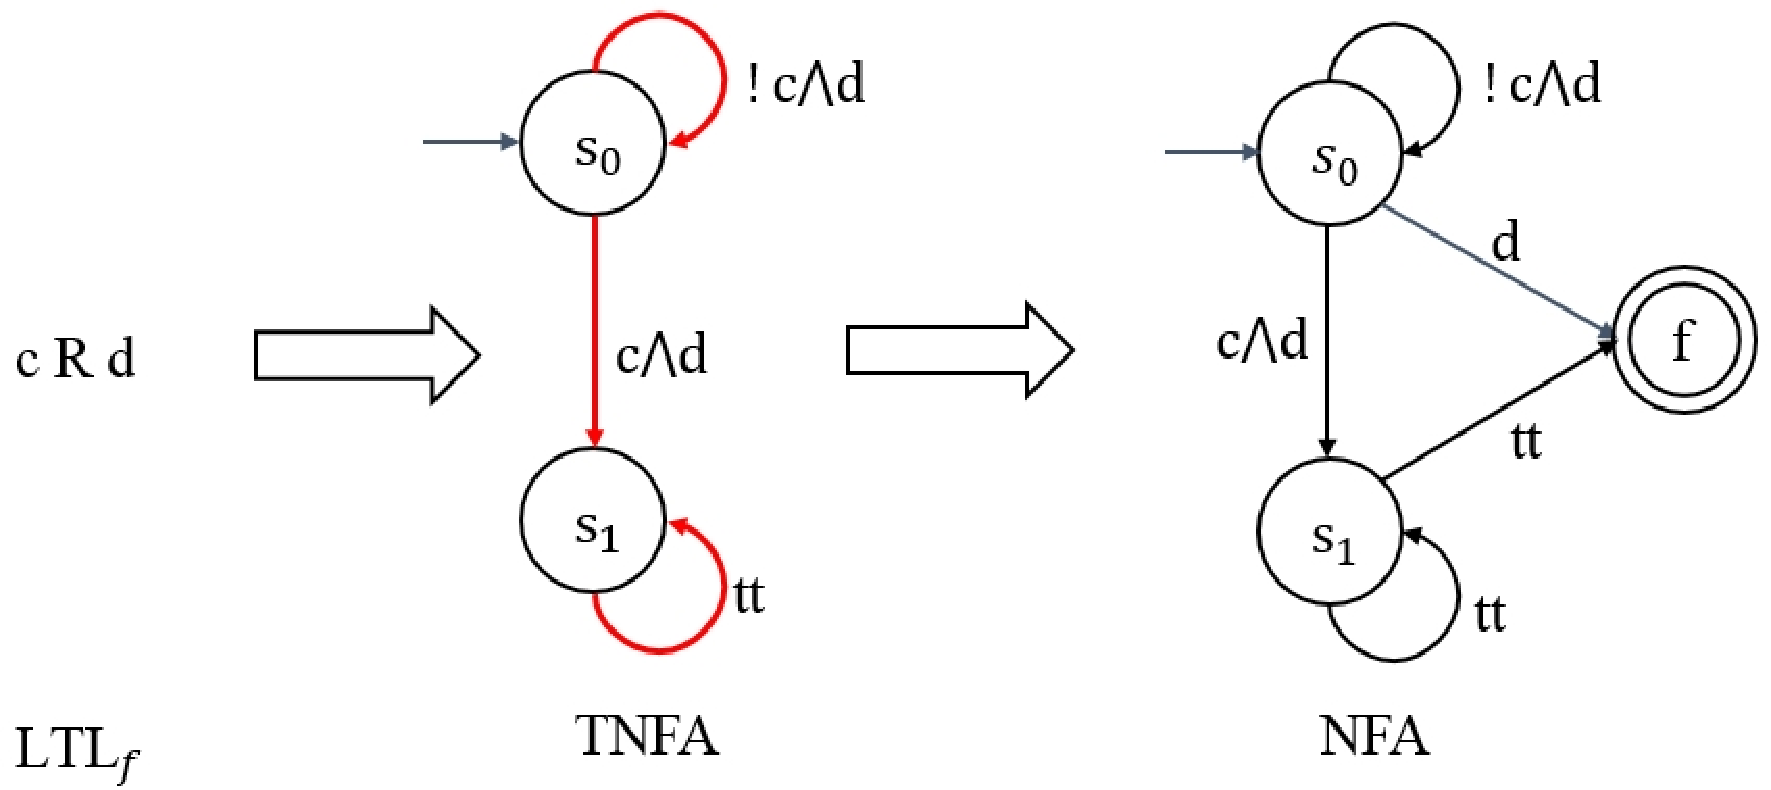
\includegraphics[scale=0.4]{overview.pdf}
  \caption{An example of our approach to construct the \NFA from an \ltlf formula. From left to right, the figure displays the input formula ($c\R d$), the equivalent transition-based \NFA (\TNFA) and the equivalent \NFA respectively. The red transitions in the \TNFA are accepting transitions.}
  \label{fig:overview}
\end{figure*}

Our approach first constructs the equivalent transition-based \NFA (\TNFA) for the input formula and then converts the \TNFA to its equivalent \NFA. A \TNFA is a special \NFA whose accepting conditions are defined over transitions instead of states. To convert a \TNFA to its equivalent \NFA, one can create a new state $f$ and add the transition $s\tran{\omega}f$ into the result \NFA for every accepting transition $s\tran{\omega}s'$ in the \TNFA. The new state $f$ is the only accepting state in the resulting \NFA. Figure \ref{fig:overview} illustrates an example of the whole translation process. 

Given an \ltlf formula $\phi$, the high-level descriptions on how to generate the equivalent \TNFA are as follows. We first convert $\phi$ to its neXt Normal Form (\XNF), which can be considered as a propositional formula over the alphabet composed of only Boolean atoms and neXt formulas. For example, the \XNF of the formula $\phi=a\R b$, which is denoted as $\xnf(\phi)$, is $b\wedge (a\vee \X(a\R b))$. Notably, the conversion cost from an \ltlf formula to its \XNF is linear to the size of the formula. Then we utilize $\xnf(\phi)^p$ to denote the propositional formula over the alphabet set $\{a, b, \X(a\R b)\}$.

Taking $\xnf(\phi)^p$ as the input, an \SAT solver is able to compute a satisfying assignment $A$, e.g., $A=\{\neg a, b, \X(a\R b)\}$. The information inside $A$ indicates that there is a transition from $\phi$ to itself with the label $\neg a\wedge b$. Analogously, the assignment $A=\{a, b, \neg \X(a\R b)\}$ tells that there is a transition from $\phi$ to $\tt$ (because there is no $\X$ element in $A$) with the label $a\wedge b$. Now $\tt$ is a new state and we continue the above process to create new transitions until no new state is generated. Finally we identify the accepting transitions, the details of which are shown below. 

Constructing the equivalent \DFA from an \ltlf formula is similar to constructing \NFA. We can also utilize the \SAT techniques to obtain a transition-based \DFA (\TDFA) directly from the input formula. The idea to generate deterministic transitions are as follows. For the given state $q$, which essentially is a set of subformulas of the input formula and can be considered as a formula as well, we use the \SAT solver to get one of the satisfying assignment $A$ of $\xnf(q)^p$ at first. From $A$ we can fix the label, denoted as $L(A)$, on the transition and then enumerate all satisfying assignments of $q$ that include $L(A)$. After that, we create a transition starting from $q$ with the label $L(A)$. Recursively applying the above procedure, all the states of the $\TDFA$ can be constructed. Finally, we present a methodology to identify the accepting transitions on the generated automaton, whose details are as below. 

From the \TDFA we can easily construct the equivalent \NFA, from which one can use the Subset Construction to create the corresponding \DFA.





\section{SAT-Based Automata Construction}

In this section, we present the construction from an \ltlf formula to the equivalent \NFA and \DFA respectively. 


\subsection{\ltlf-to-\NFA Construction}

To leverage \SAT solvers for the automata construction, we first need to consider \ltlf formulas as propositional formulas. The motivation comes from treating all temporal subformulas of $\phi$ as atomic propositions. 

\begin{definition}[Propositional Atoms]\label{def:pa}
For an \ltlf formula $\phi$, we define the set of propositional atoms, $\PA(\phi)$, recursively as follows.
\begin{itemize}
	\item If $\phi$ is an atom, Next, weak Next, Until or Release formula, $\PA(\phi)=\{\phi\}$;
	\item If $\phi = (\neg \psi)$, $\PA(\phi)= \PA(\psi)$;
	\item If $\phi = (\phi_1 \wedge \phi_2)$ or $(\phi_1 \vee \phi_2)$, $\PA(\phi) = \PA(\phi_1) \cup \PA(\phi_2)$.
\end{itemize}
\end{definition}

Consider the formula $\phi$ = $(a \wedge ((\neg c \wedge a)\U b) \wedge (c \wedge \X (a \vee b)))$ as an example. According to Definition \ref{def:pa}, we have $\PA(\phi)=\{a, c, (\neg c \wedge a)\U b), (\X (a \vee b))\}$. Now we define the propositional formula over the propositional atoms w.r.t. an \ltlf formula.

\begin{definition}[Propositional Formulas]\label{def:pf}
Given an \ltlf formula $\phi$, let $\phi^{p}$ be a propositional formula over $\PA(\phi)$. 
\end{definition}

Consider $\phi$ = $(a \wedge ((\neg c \wedge a)\U b) \wedge (c \wedge \X (a \vee b)))$. From Definition \ref{def:pf}, the corresponding propositional formula $\phi^p = (a \wedge p_1) \wedge (c \wedge p_2)$, in which $p_1, p_2$ are two Boolean variables w.r.t. the truth values of $((\neg c \wedge a)\U b)$ and $(c \wedge \X (a \vee b))$. We define the \emph{next normal form} for an \ltlf formula, whose corresponding propositional formula is the actual input of \SAT solvers.

\begin{definition}[neXt Normal Form]\label{def:xnf}
For an \ltlf formula $\phi$, we define its Next Normal Form, i.e., $\xnf(\phi)$, recursively as follows. 
\begin{itemize}
\item $\xnf(\tt) = \tt$ and $\xnf(\ff) = \ff$;
\item If $\phi$ is a literal, $\xnf(\phi) = \phi \wedge \X(\tt)$;
\item If $\phi = \X(\psi)$ or $\phi = \N(\psi)$, $\xnf(\phi) = \tt \wedge \X(\psi)$;
\item If $\phi = (\phi_1 \wedge \phi_2)$, $\xnf(\phi) = \xnf(\phi_1)\wedge\xnf(\phi_2)$;
\item If $\phi = (\phi_1 \vee \phi_2), \xnf(\phi) = \xnf(\phi_1)\vee \xnf(\phi_2)$; 
\item If $\phi = (\phi_1 \U \phi_2), \xnf(\phi) = \xnf(\phi_2) \vee (\xnf(\phi_1) \wedge \X(\phi))$; 
\item If $\phi = (\phi_1 \R \phi_2), \xnf(\phi) = \xnf(\phi)\wedge (\xnf(\phi_2) \vee \X(\phi))$.
\end{itemize}
\end{definition}

By restricting the \ltlf formula $\phi$ to the \XNF, we can obtain a satisfying assignment of $\phi^{p}$ with the help of a SAT solver.
For a satisfying assignment $A$, we define $X(A)=\{\theta\ |\ \X\theta\in A\}$ and $L(A) =\{l\ |\ l \textit{ is a literal}\}$. Also for the simple description, \textbf{we mix the usage of $X(A)$ to denote the conjunction of all elements in the set, i.e., $\bigwedge_{\psi_i\in X(A)}\psi$. The same applies to $L(A)$.}
The following lemma describes the relationship between an \ltlf formula and the satisfying assignment of its corresponding propositional formula.

\begin{lemma}\label{lem:propSat}
Given an \ltlf formula $\phi$ in the \XNF and a finite trace $\eta\in\Sigma^+$ with $|\eta|>1$, $\eta\models\phi$ holds iff there is a satisfying assignment $A$ of $\phi^p$ such that $\eta[0]\models L(A)$ and $\eta\models X(A)$.
\end{lemma}
\begin{proof}
$(\Rightarrow)$ The proof can be achieved by induction over the types of $\phi$.
\begin{itemize}
	\item if $\phi$ is a literal, Next, Unitl or Release formula, $\eta\models\phi$ implies $\eta[0]\models\phi$. Let $A=\{\phi\}$ and it is true that $\eta[0]\models L(A)$ and $\eta_1\models X(A)$ (In this situation, $X(A)\equiv \tt$); 
	\item if $\phi = \phi_1\wedge\phi_2$, $\eta\models\phi$ 
implies $\eta\models\phi_1$ and $\eta\models\phi_2$. By assumption hypothesis, there is $A_i$ of $\phi_i^p$ ($i=1,2$) such that 
$\eta[0]\models L(A_i)$ and $\eta_1\models X(A_i)$. Let $A = A_1\cup A_2$, and a consistent $A$, in which either $\psi$ or $\neg \psi$ cannot be together, 
must exists ($A$ may not be unique because $A_1$ and $A_2$ may not be unique). 
Otherwise, there is $\psi\in A_1$ and $\neg\psi\in A_2$ 
such that $\eta$ cannot model $\bigwedge A_1$ and $\bigwedge A_2$ at the same time, which is a contradiction. So $A$ is a satisfying  assignment of $\phi^p$, which leads to $\eta[0]\models L(A)$ and $\eta_1\models X(A)$. 
\item The proof for $\phi=\phi_1\vee\phi_2$ is analogous with the proof when $\phi = \phi_1\wedge\phi_2$. Also, Since $\phi$ is in \XNF, $\phi$ cannot be an Until or Release formula. The proof is done.
\end{itemize} 

$(\Leftarrow)$ $A$ is a satisfying assignment of $\phi^p$, so $A\models\phi^p$ implies $(\bigwedge A)\Rightarrow \phi$. 
Also, $\eta[0]\models L(A)$ and $\eta_i\models X(A)$ implies $\eta\models \bigwedge A$. Therefore, it is true that $\eta\models \phi$.
\end{proof}

Lemma \ref{lem:propSat} does not cover the case when $|\eta|=1$, which yields the following corollary. 

\begin{corollary}\label{coro:propSat}
Given an \ltlf formula $\phi$ in the \XNF and a finite trace $\eta\in\Sigma^+$ with $|\eta|=1$, $\eta\models\phi$ holds implies there is a satisfying assignment $A$ of $\phi^p$ such that $\eta[0]\models L(A)$.
\end{corollary}
\begin{proof}
The proof is similar to that of Lemma \ref{lem:propSat} for the ($\Rightarrow$) direction, the details of which are omitted here.
\end{proof}
  
Informally speaking, if $\phi$ is a state in the \NFA, $X(\xnf(\phi)^p)$ represents one of its successors and $L(\xnf(\phi)^p)$ represents the label on the transition from $\phi$ to $X(\xnf(\phi)^p)$. Now we present the construction from an \ltlf formula to its equivalent transition-based \NFA. 

   
\begin{definition}[Transition-based NFA (\TNFA)]\label{def:ltlf2nfa} 
Given an \ltlf formula $\phi$, the corresponding transition-based \NFA ${\A_{\phi}}^{tn}$ is defined as a tuple $(\Sigma, S, \rho, s_0, T)$ such that
\begin{itemize}
	\item $\Sigma = 2^{L}$ is the set of alphabet, where $L$ is the literal set of $\phi$;
	\item $S\subseteq 2^{\cl(\phi)}$ is the set of states;
	\item $\rho:  S \times \Sigma \to 2^S$ is the transition function, where $s_2 \in \rho(s_1, \omega) (\omega \in \Sigma)$ holds iff there is a satisfying assignment $A$ of $\xnf(s_1)^p$ such that $s_2 = X(A)$ and $\omega\models L(A)$;
	\item $s_0 = \{\phi \}$ is the initial state;
	\item $T\subseteq \rho$ is the set of accepting transitions. A transition $s_1\tran{\omega}s_2$ is in $T$ iff $\omega\models s_1$ holds. 
\end{itemize}
\end{definition}

As Definition \ref{def:ltlf2nfa} shows, a state in the \NFA is a set of subformulas of the input $\phi$. For the simple description, \textbf{we mix the usage of a state $s$ such that it can also represent a Boolean formula $\bigwedge_{\psi_i\in s}\psi_i$, i.e., the conjunction of all subformulas in $s$.} 

A run $r$ of the transition-based \NFA ${\A_{\phi}}^{tn}$ on $\eta$ is a finite state sequence $s_0 s_1\ldots$ such that $s_0$ is the initial state and $s_{i+1}\in\rho(s_i,\omega_i)$ for $0\leq i < |\eta|$. $\eta$ is accepted by ${\A_{\phi}}^{tn}$ iff there is a run $r$ of ${\A_{\phi}}^{tn}$ on $\eta$ which ends with some accepting transition in $T$. 

Since in Definition \ref{def:ltlf2nfa}, the satisfaction of a finite trace with length one to an \ltlf formula is used to determine the accepting conditions, we introduce the following theorem to show that this process can be achieved in a much easier way than the regular satisfaction check in which the finite trace can have an arbitrary length.

\begin{theorem}\label{thm:oneSat}
Given a finite trace $\eta \in \Sigma^{+}$ with $|\eta|=1$, and an \ltlf formula $\phi$, it is true that $\eta \models \phi$ holds iff
\begin{itemize}
	\item $\phi$ is $\tt$; or 
	\item $\phi \in\eta$ when $\phi$ is a literal; or
	%\item If $\phi=\X \psi$, then return false;
	\item $\phi=\N \psi$ is a weak Next formula; or
	\item $\eta \models \phi_{2}$ holds when $\phi=\phi_{1} \U \phi_{2}$ is an Until formula; or  
	\item $\eta \models \phi_{2}$ holds when $\phi=\phi_{1} \R \phi_{2}$ is a Release formula; or
	\item $\eta \models \phi_{1}$ and $\eta \models \phi_{2}$ hold when $\phi=\phi_{1} \wedge \phi_{2}$; or
	\item $\eta \models \phi_{1}$ or $\eta \models \phi_{2}$ holds when $\phi=\phi_{1} \vee \phi_{2}$.
\end{itemize}
\end{theorem}

\begin{proof}
The lemma is self-explained which can be derived from the semantics of \ltlf.
\end{proof}

We present the following theorem to guarantee the correctness of our construction. 

\begin{theorem}\label{thm:ltlf2nfa}
Given an \ltlf formula $\phi$ and the \TNFA ${\A_{\phi}}^{tn}$ constructed by Definition \ref{def:ltlf2nfa}, a finite trace $\eta\models\phi$ holds iff $\eta$ is accepted by ${\A_{\phi}}^{tn}$. 
\end{theorem}
\begin{proof}
Assume $\eta = \omega_0\omega_1\ldots\omega_n$ ($n\geq 0$). 

($\Leftarrow$) We prove by induction over the values of $n$.
\begin{itemize}
	\item According to Definition \ref{def:ltlf2nfa}, $\eta$ is accepted by ${\A_{\phi}}^{tn}$ implies that there is a run $r=s_0s_1\ldots s_n s_{n+1}$ of ${\A_{\phi}}^{tn}$ on $\eta$ such that $\omega_n\models s_{n}$. So basically when $k = n$, it holds that $\eta_k\models s_k$;
	\item Inductively, assume $\eta_k\models s_k$ holds for $0<k\leq n$. Because $s_{k-1}\tran{\omega_{k-1}}s_k$ is a transition in the \TNFA and $\eta_k\models s_k$ holds, the set $A_{k-1} = \omega_{k-1}\cup \{\X\theta | \theta\in s_k\}$ is a satisfying assignment of $\xnf(s_{k-1})^p$, from Definition \ref{def:ltlf2nfa}. Then based on Lemma \ref{lem:propSat} and since $\eta_{k-1}=\omega_{k-1}\cdot\eta_k$ is true, we have that $\eta_{k-1}\models s_{k-1}$.
\end{itemize}
When $k=0$, we prove that $\eta (=\eta_0)\models \phi (=s_0)$ is true.

($\Rightarrow$) We first prove that $\eta\models\phi$ implies there is a run $r$ of ${\A_{\phi}}^{tn}$ on $\eta$. 
If $n = 0$, Corollary \ref{coro:propSat} shows that there is a satisfying assignment $A$ of $\xnf(\phi)^p$ such that $\eta[0]\models L(A)$. From Definition \ref{def:ltlf2nfa}, $\phi\tran{\eta[0]}X(A)$ is a transition of the \TNFA. As a result, there is a run $r=s_0(=\phi)s_1(=X(A))$ of ${\A_{\phi}}^{tn}$ on $\eta$.
 
If $n>0$, according to Lemma \ref{lem:propSat}, $\eta\models\phi$ implies there is a satisfying assignment $A$ of $\xnf(\phi)^p$ such that $\omega_0\models L(A)$ and $\eta_1\models X(A)$. From Definition \ref{def:ltlf2nfa}, $\phi (=s_0)\tran{\omega_0}X(A) (=s_1)$ is a transition in the \TNFA. Recursively applying the above process to $\eta_i\models s_i(i\geq 1)$, one can prove there is a transition $s_i\tran{\omega_i}s_{i+1}$ in the \TNFA. As a result, we have $\eta\models\phi$ implies there is a run $r$ of ${\A_{\phi}}^{tn}$ on $\eta$.  

Now we prove that the run $r$ is an accepting run. If $n=0$, the run $r$ is $s_0s_1$ such that $\eta[0]\models s_0(=\phi)$ holds. According to Definition \ref{def:ltlf2nfa}, the transition $s_0\tran{\eta[0]}s_1$ is an accepting transition. As a result, $r$ is an accepting run and $\eta$ is accepted by ${\A_{\phi}}^{tn}$.

If $n>0$, we can also prove that for the run $r=s_0s_1\ldots s_n s_{n+1}$, $s_n\tran{\omega_n}s_{n+1}$ is an accepting transition, due to the fact that $\omega_n\models s_n$. The proof is done.
\end{proof}

We discuss the upper bound of the generated \TNFA in the following theorem.

\begin{theorem}\label{thm:tnfaBound}
For an \ltlf formula $\phi$, the size of the corresponding $\TNFA$ ${\A_{\phi}}^{tn}$ generated by Definition \ref{def:ltlf2nfa} is at most $2^{|cl(\phi)|}$.
\end{theorem}
\begin{proof}
	The proof is straightforward as every state in ${\A_{\phi}}^{tn}$ is from $s^{cl(\phi)}$, according to Definition \ref{def:ltlf2nfa}.
\end{proof}

We have shown the construction from an \ltlf formula to its equivalent \TNFA. The following theorem indicates that there is a trivial way to convert a \TNFA to its equivalent \NFA. 

\begin{theorem}\label{tnfa2nfa}
For a \TNFA $\A^{tn}$, there is a \NFA $\A^n$ such that $\eta$ is accepted by $\A^{tn}$ iff $\eta$ is accepted by $\A^n$, for $\eta\in \Sigma^+$. 
\end{theorem}
\begin{proof}
Assume $\A^{tn}=(\Sigma, S, \rho, s_0, T)$ and one can construct the \NFA $\A^{n} = (\Sigma, S', \rho', s_0, F)$ such that 
\begin{itemize}
	\item $S' = S\cup \{f\}$ where $f$ is a new and the only accepting state in $\A^n$; and 
	\item the transition function $\rho'$ satisfies $s_2\in \rho'(s_1,\omega)$ holds iff $s_2\in \rho(s_1, \omega)$ holds when $s_2\not = f$; otherwise, there is a transition $s_1\tran{\omega}s_3$ in $T$. 
	\item $F=\{f\}$.
\end{itemize}
We consider as follows to prove the equivalence of $\A^{tn}$ and $\A^n$: On one hand, every accepting run of $\A^{tn}$ which ends with an accepting transition in $T$ can also be an accepting run of $\A^n$ which ends with the accepting state $f$. On the other hand, every accepting run of $\A^{n}$ which ends with the accepting state $f$ can also be an accepting run of $\A^{tn}$ which ends with an accepting transition in $T$.
\end{proof}




\subsection{\ltlf-to-(T)\DFA Construction}

Based on the \NFA construction in the previous section, the equivalent \DFA w.r.t the \ltlf formula may be obtained by applying the Subset Construction to the generated \NFA. However, such \DFA construction is not on the fly, as it has to be postponed until the \NFA is fully generated. Inspired from Definition \ref{def:ltlf2nfa}, which enables to construct the \TNFA on the fly, we present here an on-the-fly construction directly from the \ltlf formula to the equivalent transition-based \DFA (\TDFA). 

Let $\phi$ be a propositional formula and we utilize $\allsat(\phi)$ to represent the set of all satisfying assignments of $\phi$. Given a literal set $L$, we also define the projection of $\allsat(\phi)$ under $L$, i.e., $\allsat(\phi)_{|L}$, which is a subset of $\allsat(\phi)$ such that $A\supseteq L$ iff $A\in \allsat(\phi)_{|L}$. Informally speaking, $\allsat(\phi)_{|L}$ represents exactly the set of satisfying assignments of $\phi$ including $L$. Now we are ready to present the \TDFA construction. 

\begin{definition}[Transition-based \DFA]\label{def:ltlf2dfa}
Given an \ltlf formula $\phi$, the corresponding transition-based \DFA ${\A_{\phi}}^{td}$ is defined as a tuple $(\Sigma, Q, \delta, q_0, T^d)$ such that
\begin{itemize}
	\item $\Sigma = 2^{L}$ is the set of alphabet, where $L$ is the literal set of $\phi$;
	\item $Q\subseteq 2^{2^{\cl(\phi)}}$ is the set of states;
	\item $\delta:  Q \times \Sigma \to Q$ is the transition function, where $q_2 = \delta(q_1, \omega) (\omega \in \Sigma)$ holds iff $q_2=\{X(A) | A\in\allsat(\xnf(q_1)^p)_{|\omega}\}$;
	\item $q_0 = \{\{\phi \}\}$ is the initial state;
	\item $T^d\subseteq \delta$ is the set of accepting transitions. A transition $q_1\tran{\omega}q_2$ is in $T^d$ iff there is a $s\in q_1$ such that $\omega\models s$ holds. 
\end{itemize}

\end{definition}

Analogous to the state representation of the \TNFA, we mix the usage of a state $q$ in the \TDFA such that $q$ also represents the \ltlf formula $\bigvee_{s\in q}\bigwedge_{\psi\in s}\psi$. 

A run $r$ of the transition-based \DFA ${\A_{\phi}}^{td}$ on $\eta$ is a finite state sequence $q_0 q_1\ldots$ such that $q_0$ is the initial state and $q_{i+1} = \delta(q_i,\omega_i)$ for $0\leq i < |\eta|$. Since ${\A_{\phi}}^{td}$ is deterministic, the run $r$ on $\eta$ is unique. $\eta$ is accepted by ${\A_{\phi}}^{td}$ iff the only run $r$ of ${\A_{\phi}}^{tn}$ on $\eta$ ends with some accepting transitions in $T^d$. The following theorem guarantees the correctness of the \TDFA construction shown in Definition \ref{def:ltlf2dfa}. 

\begin{theorem}
Given an \ltlf formula $\phi$ and the \TDFA ${\A_{\phi}}^{td}$ constructed by Definition \ref{def:ltlf2dfa}, a finite trace $\eta\models\phi$ holds iff $\eta$ is accepted by ${\A_{\phi}}^{td}$. 
\end{theorem}
\begin{proof}
Assume ${\A_{\phi}}^{tn}$ is the \TNFA constructed by Definition \ref{def:ltlf2nfa} w.r.t $\phi$. Intuitively, ${\A_{\phi}}^{td}$ from Definition \ref{def:ltlf2dfa} is equivalent to the \TDFA constructed by applying the Subset Construction to ${\A_{\phi}}^{tn}$. However, the Subset Construction is not standardized for transition-based finite automata such that the above intuition is not straightforward. Instead, we follow the proof of Theorem \ref{thm:ltlf2nfa} and prove this theorem analogously as follows.

Assume $\eta = \omega_0\omega_1\ldots\omega_n$ ($n\geq 0$). 

($\Leftarrow$) 
According to Definition \ref{def:ltlf2dfa},  $\eta$ accepted by ${\A_{\phi}}^{td}$ implies that there is a run $r=q_0q_1\ldots q_n q_{n+1}$ of ${\A_{\phi}}^{td}$ on $\eta$ such that $q_{n}\tran{\omega_{n}}q_{n+1} \in \delta$ and $\omega_n\models s$ for some $s\in q_n$.
To prove $\eta$ is accepted by ${\A_{\phi}}^{td}$ implies $\eta\models\phi$ holds, we only need to prove $\eta$ is accepted by ${\A_{\phi}}^{td}$ implies $\eta_{n-i}\models q_{n-i}$ for\ i=0...n. Then we could have $\eta (=\eta_0)\models \phi (=q_0)$ when $i=n$.

We prove by induction over the values of $i$.
\begin{itemize}
	\item By Definition \ref{def:ltlf2dfa}, we have that $\omega_n\models s$ for some $s\in q_n$. Since $q_n = \bigvee_{s\in q_n}\bigwedge_{\psi\in s}\psi$, it is true that $s\implies q_n$ for every $s\in q_n$. So $\omega_n\models s$ implies $\omega_n\models q_n$, which means basically when $i = 0$, it holds that $\eta_{n-0}\models q_{n-0}$;
	\item Inductively, assume $\eta_{n-i}\models q_{n-i}$ holds by satisfying $\eta_{n-i}\models s$ for some $s\in q_{n-i}$ ($0<i\leq n$). Because $q_{n-i-1}\tran{\omega_{n-i-1}}q_{n-i}$ is a transition in the \TDFA and $\eta_{n-i}\models q_{n-i}$ holds, the set $A_{n-i-1} = \omega_{n-i-1}\cup \{\X\theta | \theta\in s\}$ is a satisfying assignment of $\xnf(q_{n-i-1})^p$ in $\allsat(\xnf(q_{n-i-1})^p)_{|\omega_{n-i-1}}$, from Definition \ref{def:ltlf2dfa}. Then based on Lemma \ref{lem:propSat} and since $\eta_{n-i-1}=\omega_{n-i-1}\cdot\eta_{n-i}$ is true, we have that $\eta_{n-i-1}\models q_{n-i-1}$.
\end{itemize}

($\Rightarrow$) We first prove that $\eta\models\phi$ implies that there is a run $r$ of ${\A_{\phi}}^{td}$ on $\eta$. 
If $n = 0$, Corollary \ref{coro:propSat} shows that there is a satisfying assignment $A$ of $\xnf(\phi)^p$ such that $\eta[0]\models L(A)$. From Definition \ref{def:ltlf2dfa}, $\phi\tran{\eta[0]}q$, where $q=\{X(A') | A'\in\allsat(\xnf(\phi)^p)_{|L(A)}\}$, is a transition of the \TDFA. As a result, there is a run $r=q_0(=\phi)q$ of ${\A_{\phi}}^{td}$ on $\eta$.
 
If $n>0$, according to Lemma \ref{lem:propSat}, $\eta\models\phi$ implies there is a satisfying assignment $A$ of $\xnf(\phi)^p$ such that $\omega_0\models L(A)$ and $\eta_1\models X(A)$. From Definition \ref{def:ltlf2dfa}, $\phi (=q_0)\tran{\omega_0}q_1$, where $q_1=\{X(A') | A'\in\allsat(\xnf(\phi)^p)_{|\omega_0}\}$, is a transition in the \TDFA. Recursively applying the above process to $\eta_i\models q_i(i\geq 1)$, one can prove there is a transition $q_i\tran{\omega_i}q_{i+1}$ in the \TDFA. As a result, we have $\eta\models\phi$, which implies there is a run $r$ of ${\A_{\phi}}^{td}$ on $\eta$.  

Now we have that $\eta\models\phi$ implies there is a run $r=q_0...q_n q_{n+1}$ of ${\A_{\phi}}^{td}$ on $\eta$ and $\eta_i\models q_i\ for\ i=0...n$. When $i=n$, $\eta_n\models q_n$ i.e., $\omega_n\models q_n$ holds. According to Definition \ref{def:ltlf2dfa}, the transition $q_n\tran{\omega_n}q_{n+1}$ is an accepting transition. As a result, $r$ is an accepting run and $\eta$ is accepted by ${\A_{\phi}}^{td}$.
\end{proof}

We now discuss the upper bound of the generated \TDFA in the following theorem.

\begin{theorem}\label{thm:tdfaBound}
For an \ltlf formula $\phi$, the size of the corresponding $\TDFA$ ${\A_{\phi}}^{td}$ generated by Definition \ref{def:ltlf2dfa} is at most $2^{2^{|cl(\phi)|}}$.
\end{theorem}
\begin{proof}
	The proof is straightforward as every state in ${\A_{\phi}}^{td}$ is from $2^{2^{cl(\phi)}}$, according to Definition \ref{def:ltlf2dfa}.
\end{proof}

It should be noted that, the conversion from a \TNFA to its equivalent \NFA shown in Theorem \ref{thm:tnfa2nfa} is not applicable to that from a \TDFA to its equivalent \DFA. In fact, the resulting automaton can only be an \NFA. One still has to apply the Subset Construction to the \NFA for the equivalent \DFA. However, we argue that for real application purposes, such as \ltlf synthesis that requires \DFA, working on \TDFA has the same or even better performance. Currently, this is out of this paper's scope.  


\section{Approach Overview}
Given an $LTL_f$ formula $\phi$, there is a \NFA $A_{\phi}$ which accepts exactly the same language as $\phi$. To construct the nondeterministic finite automaton (\NFA) for an $ LTL_f$ formula $\phi$, our approach first constructs the corresponding transition-based \NFA, then converts the \TNFA to its equivalent \NFA. The following two subsections will describe this process. The first subsection describes the algorithm of \ltlf-to-\TNFA. The second subsection describes the algorithm of \TNFA-to-\NFA.

\subsection{\ltlf-to-\TNFA}
Given an  $ LTL_f$ formula, We define the construction of the \TNFA  as follows: \\
  \begin{algorithm}[H]
    \SetAlgoNoLine
 \SetKwInOut{Input}{\textbf{Input}}\SetKwInOut{Output}{\textbf{Output}}
 \Input{ An $ LTL_f$ formula $\phi$\\}
    \Output{ TNFA $A^{tn}$\\}
    \BlankLine
 $to\_process:= \{\xnf(\phi)\}$\\
 $xnf(\phi)$ is the initial state in S\\
\textbf{while} $to\_process$ is not empty \textbf{do} \\
\ cur =  $to\_process$.front;  \\
\quad  \textbf{while} true \textbf{do} \\
\qquad   \textbf{if} cur is not satisfiable  \textbf{then} \{ \\
\qquad \quad $to\_process$.pop; \\
\qquad \quad break;     \}\\
 \qquad  next = $\rho(cur, label)$ \\
\qquad\textbf{if} next is not in existing \textbf{then} \{ \\
\qquad \quad $to\_process$.push($next$); \\
\qquad \quad existing.push($next$); \\
\qquad  \quad add the state $next$ to S\\
\qquad  add the transition $cur\tran{label}next$ to T
 \caption{Construction of the \TNFA}
\end{algorithm}

The algorithm constructs the transition system on-the-fly. The initial state is set to be $\{\phi\}$, which is the input formula. $to\_process$ is used to store a collection of states to be processed. Visited states are stored in $existing$. $front$ is used to describe the first element of an array. In a transition $s_1\tran{\omega}s_2$, $\omega$ is the $label$, $s_2$ is the $next$ state. \\
In this algorithm, we first convert the input formula into its Next Normal Form, i.e., $\xnf(\phi)$. Then we use \SAT solvers to check if $\xnf(\phi)$ is satisfiable. If the answer is true, proceed to the next step, and if the answer is false, stop. After that, we leverage $\SAT solvers$ to get a transition $cur\tran{label}next$, and then we check if the state $next$ has been processed. If the answer is true, then we add the transition to ${A_{\phi}}^{tn}$, otherwise, the state $next$ will be added to  $to\_process$,existing and ${A_{\phi}}^{tn}$ respectively.


\subsection{\TNFA-to-\NFA}  
In the previous section, we constructed the state and transition of the \TNFA. This section will focus on the conversion from \TNFA-to-\NFA, with the addition of accepting states. The algorithm is stated as follows:\\

\IncMargin{1em}
 \begin{algorithm}[H]
    \SetAlgoNoLine
 \SetKwInOut{Input}{\textbf{Input}}\SetKwInOut{Output}{\textbf{Output}}
 \Input{ \TNFA $A^{tn}$\\}
    \Output{  \NFA $A^{n}$}
    \BlankLine
 
\qquad  $S' = S\cup \{f\}$   \\
\qquad  \textbf{for} state $s_2$ in S \\
\qquad \quad \textbf{if} $s_2\not = f$ and $s_2\in \rho(s_1, \omega)$\textbf{then} \{  \\
\qquad \qquad  $\rho'(s_1,\omega)$ = $\rho(s_1, \omega)$ \} \\
\qquad \quad \textbf{else} \{  \\
\qquad \qquad add a transition $s_1\tran{\omega}s_3$ in $\rho'$
\} \\
 \caption{\TNFA-to-\NFA}
\end{algorithm}

This algorithm converts the \TNFA to \NFA. S is the set of states in \TNFA, while $S'$ is the set of states in \NFA. f is the only accepting state in \NFA $A^{n}$. \\





\section{ Conclusions}

Although a conclusion may review the main points of the paper, do not replicate the abstract as the conclusion. A conclusion might elaborate on the importance and results of the work, and/or suggest applications and extensions.

\vspace{2mm}

 

\begin{thebibliography}{99}
\footnotesize
\itemsep=-3pt plus.2pt minus.2pt
\baselineskip=13pt plus.2pt minus.2pt
\bibitem{1}Sayah J Y, Kime C R. Test scheduling in high performance VLSI system implementations. {\it IEEE Trans. Computers}, 1992, 41(1): 52-67.  [\textcolor{blue}{example for journal paper}]


\end{thebibliography}

\label{last-page}
\end{multicols}
\end{document}

